\documentclass[border=10pt]{standalone}
\usepackage{pgfplots}
\pgfplotsset{compat=1.18}

\begin{document}
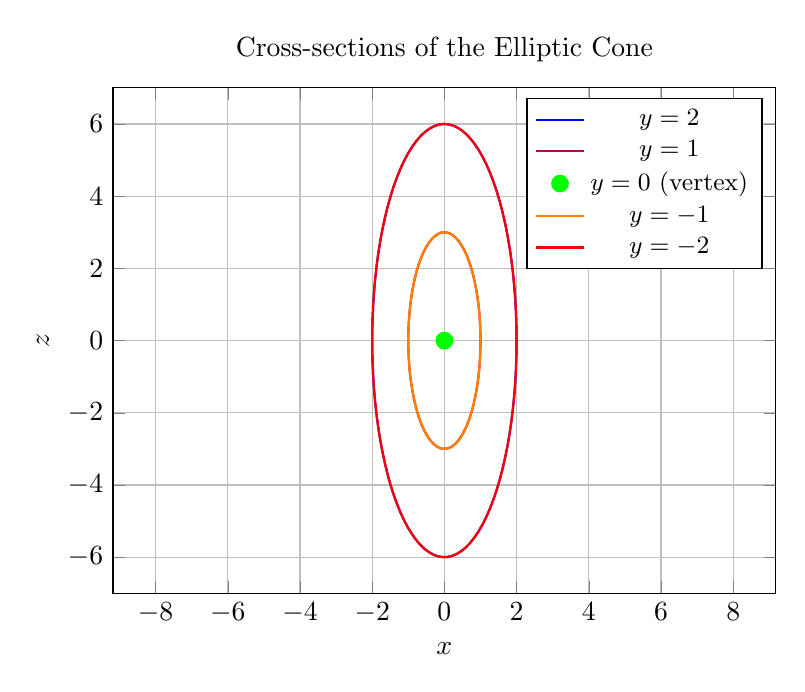
\begin{tikzpicture}
\begin{axis}[
    xlabel={$x$},
    ylabel={$z$},
    title={Cross-sections of the Elliptic Cone},
    domain=0:360,
    samples=100,
    axis equal,
    grid=major,
    width=10cm,
    height=8cm,
    xmin=-7,
    xmax=7,
    ymin=-7,
    ymax=7,
    legend style={at={(0.98,0.98)}, anchor=north east, font=\small}
]

% Cross-section at y = 2 (blue)
\addplot[blue, thick] ({2*cos(x)}, {6*sin(x)});
\addlegendentry{$y=2$}

% Cross-section at y = 1 (purple)
\addplot[purple, thick] ({1*cos(x)}, {3*sin(x)});
\addlegendentry{$y=1$}

% Cross-section at y = 0 (point)
\addplot[green, only marks, mark=*, mark size=3pt] coordinates {(0,0)};
\addlegendentry{$y=0$ (vertex)}

% Cross-section at y = -1 (orange)
\addplot[orange, thick] ({1*cos(x)}, {3*sin(x)});
\addlegendentry{$y=-1$}

% Cross-section at y = -2 (red)
\addplot[red, thick] ({2*cos(x)}, {6*sin(x)});
\addlegendentry{$y=-2$}

\end{axis}
\end{tikzpicture}
\end{document}